\documentclass[a4paper]{article}
\usepackage{vntex}
%\usepackage[english,vietnam]{babel}
%\usepackage[utf8]{inputenc}
%\usepackage[utf8]{inputenc}
%\usepackage[francais]{babel}
\usepackage{a4wide,amssymb,epsfig,latexsym,multicol,array,hhline,fancyhdr}
\usepackage{booktabs}
\usepackage{amsmath}
\usepackage{lastpage}
\usepackage[lined,boxed,commentsnumbered]{algorithm2e}
\usepackage{enumerate}
\usepackage{color}
\usepackage{graphicx}							% Standard graphics package
\usepackage{array}
\usepackage{tabularx, caption}
\usepackage{multirow}
\usepackage[framemethod=tikz]{mdframed}% For highlighting paragraph backgrounds
\usepackage{multicol}
\usepackage{rotating}
\usepackage{graphics}
\usepackage{geometry}
\usepackage{setspace}
\usepackage{epsfig}
\usepackage{tikz}
\usepackage{listings}
\usetikzlibrary{arrows,snakes,backgrounds}
\usepackage{hyperref}
\hypersetup{urlcolor=blue,linkcolor=black,citecolor=black,colorlinks=true} 
%\usepackage{pstcol} 								% PSTricks with the standard color package

\newtheorem{theorem}{{\bf Định lý}}
\newtheorem{property}{{\bf Tính chất}}
\newtheorem{proposition}{{\bf Mệnh đề}}
\newtheorem{corollary}[proposition]{{\bf Hệ quả}}
\newtheorem{lemma}[proposition]{{\bf Bổ đề}}

\everymath{\color{blue}}
%\usepackage{fancyhdr}
\setlength{\headheight}{40pt}
\pagestyle{fancy}
\fancyhead{} % clear all header fields
\fancyhead[L]{
 \begin{tabular}{rl}
    \begin{picture}(25,15)(0,0)
    \put(0,-8){
\includegraphics[width=8mm, height=8mm]{images/logoITSGUsmall.png}}
    %\put(0,-8){\epsfig{width=10mm,figure=hcmut.eps}}
   \end{picture}&
	%\includegraphics[width=8mm, height=8mm]{hcmut.png} & %
	\begin{tabular}{l}
		\textbf{\bf \ttfamily Trường Đại học Sài Gòn}\\
		\textbf{\bf \ttfamily Khoa Công Nghệ Thông Tin}
	\end{tabular} 	
 \end{tabular}
}
\fancyhead[R]{
	\begin{tabular}{l}
		\tiny \bf \\
		\tiny \bf 
	\end{tabular}  }
\fancyfoot{} % clear all footer fields
\fancyfoot[L]{\scriptsize \ttfamily Bài tập lớn môn Phát triển phần mềm mã nguồn mở - Niên khóa 2023-2024}
\fancyfoot[R]{\scriptsize \ttfamily Trang {\thepage}/\pageref{LastPage}}
\renewcommand{\headrulewidth}{0.3pt}
\renewcommand{\footrulewidth}{0.3pt}


%%%
\setcounter{secnumdepth}{4}
\setcounter{tocdepth}{3}
\makeatletter
\newcounter {subsubsubsection}[subsubsection]
\renewcommand\thesubsubsubsection{\thesubsubsection .\@alph\c@subsubsubsection}
\newcommand\subsubsubsection{\@startsection{subsubsubsection}{4}{\z@}%
                                     {-3.25ex\@plus -1ex \@minus -.2ex}%
                                     {1.5ex \@plus .2ex}%
                                     {\normalfont\normalsize\bfseries}}
\newcommand*\l@subsubsubsection{\@dottedtocline{3}{10.0em}{4.1em}}
\newcommand*{\subsubsubsectionmark}[1]{}
\makeatother

\definecolor{dkgreen}{rgb}{0,0.6,0}
\definecolor{gray}{rgb}{0.5,0.5,0.5}
\definecolor{mauve}{rgb}{0.58,0,0.82}

\lstset{frame=tb,
	language=Matlab,
	aboveskip=3mm,
	belowskip=3mm,
	showstringspaces=false,
	columns=flexible,
	basicstyle={\small\ttfamily},
	numbers=none,
	numberstyle=\tiny\color{gray},
	keywordstyle=\color{blue},
	commentstyle=\color{dkgreen},
	stringstyle=\color{mauve},
	breaklines=true,
	breakatwhitespace=true,
	tabsize=3,
	numbers=left,
	stepnumber=1,
	numbersep=1pt,    
	firstnumber=1,
	numberfirstline=true
}

\begin{document}

\begin{titlepage}
\begin{center}
TRƯỜNG ĐẠI HỌC SÀI GÒN \\
KHOA CÔNG NGHỆ THÔNG TIN
\end{center}
\vspace{1cm}

\begin{figure}[h!]
\begin{center}

\includegraphics[width=3cm]{images/logoITSGUsmall.png}
\end{center}
\end{figure}

\vspace{1cm}


\begin{center}

\vspace{0.3 cm}
{\textbf{{\Large PHÁT TRIỂN PHẦN MỀM MÃ NGUỒN MỞ}}}\\
\vspace{0.3 cm}

~~\\
\Large Phát triển game cờ Gomoku 2 người chơi bằng Pygame và Socket server\\
\end{center}

\vspace{3cm}

\begin{tabbing}
        \hspace{4 cm}\=\kill
        \> GVHD: TỪ LÃNG PHIÊU \\ 
        \> SV: NGUYỄN THÀNH LỘC - 3120410292 \\
        \> SV: NGUYỄN HOÀI LỘC - 3120410291
        
\end{tabbing}

\vspace{3.5 cm}


\begin{center}
{\footnotesize TP. HỒ CHÍ MINH, THÁNG 5/2024}
\end{center}
\end{titlepage}


\thispagestyle{empty}

\newpage
\tableofcontents
\newpage

%%%%%%%%%%%%%%%%%%%%%%%%%%%%%%%%%


%%%%%%%%%%%%%%%%%%%%%%%%%%%%%%%%%
\section{GIỚI THIỆU ĐỀ TÀI}
    Trong thời đại kỹ thuật số ngày nay, trò chơi trực tuyến không chỉ là một hình thức giải trí phổ biến mà còn là một cách tuyệt vời để kết nối và giao lưu giữa mọi người trên toàn thế giới. Với sự phát triển không ngừng của công nghệ mạng, việc tạo ra các trò chơi trực tuyến chất lượng và hấp dẫn đã trở thành một mục tiêu quan trọng của nhiều nhà phát triển phần mềm. \\
    \\
    Trong bối cảnh này, việc sử dụng mã nguồn mở đã trở thành một xu hướng phổ biến. Mã nguồn mở không chỉ mang lại sự linh hoạt và tính bảo mật mà còn khuyến khích sự hợp tác và đóng góp từ cộng đồng lập trình viên toàn cầu. Điều này mở ra cơ hội cho việc phát triển các ứng dụng và trò chơi mới mẻ, đồng thời thúc đẩy sự phát triển của ngành công nghiệp phần mềm. \\
    \\
    Trong bối cảnh này, đề tài của chúng em là "Phát triển game cờ Gomoku 2 người chơi bằng Pygame và Socket". Trong dự án này, chúng em sẽ kết hợp giữa việc tạo ra một trò chơi cổ điển như Gomoku với việc sử dụng các công nghệ mã nguồn mở như Python và sử dụng Socket server tạo kết nối cho phép họ chơi trò chơi Gomoku với nhau qua mạng LAN. Ngoài ra còn sử dụng tích hợp thuật toán Minimax và Alpha-Beta Pruning để tạo ra một máy đánh cờ. Qua đó, không chỉ khám phá sức mạnh của phần mềm mã nguồn mở mà còn tạo ra một sản phẩm giải trí độc đáo và thú vị. \\
    \\
    Qua dự án này, các mục tiêu được chúng em đề ra là:
    
    \begin{itemize}
        \item Nắm vững kiến thức về lập trình game sử dụng Pygame và xử lý sự kiện.
        \item Hiểu về cách thiết kế giao diện người dùng cho trò chơi.
        \item Học cách sử dụng Socket để thiết lập kết nối mạng giữa các máy tính.
        \item Xây dựng một bot AI để đánh nhau với người chơi.
    \end{itemize}
    
\newpage
%%%%%%%%%%%%%%%%%%%%%%%%%%%%%%%%%
\section{CÁC CÔNG NGHỆ SỬ DỤNG}

\subsection{Ngôn ngữ lập trình Python}
    Python là một lựa chọn phù hợp cho việc phát triển ứng dụng này vì có nhiều lợi ích như:
\begin{itemize}
    \item Có cú pháp đơn giản và dễ đọc, giúp tăng tính đảm bảo và hiểu biết của đội ngũ phát triển.
    \item Python là một ngôn ngữ đa năng và mạnh mẽ, có thể được sử dụng cho nhiều mục đích khác nhau từ phát triển web, xử lý dữ liệu, đến trí tuệ nhân tạo và học máy.
    \item Có một cộng đồng lớn và tích cực, cung cấp nhiều thư viện và framework hữu ích giúp việc phát triển ứng dụng trở nên nhanh chóng và dễ dàng hơn.
    \item Miễn phí và mã nguồn mở, giúp tiết kiệm chi phí phát triển và tạo điều kiện thuận lợi cho sự mở rộng và phát triển của dự án trong tương lai.
\end{itemize}

\subsection{Pygame}
Sử dụng Pygame để xây dựng giao diện ứng dụng mang lại nhiều ưu điểm quan trọng.
\begin{itemize}
    \item Pygame là một thư viện mã nguồn mở cho Python được thiết kế để phát triển các ứng dụng và trò chơi đa phương tiện. Dựa trên SDL (Simple DirectMedia Layer), Pygame cung cấp các công cụ và API cho việc vẽ đồ họa, xử lý sự kiện, âm thanh và vận động, giúp người phát triển dễ dàng tạo ra các trò chơi và ứng dụng có giao diện đồ họa.
    \item Dễ học và sử dụng: Pygame được thiết kế để đơn giản và dễ hiểu, phù hợp cho cả người mới bắt đầu và những người có kinh nghiệm trong lập trình Python.
    \item Hỗ trợ đa nền tảng: Pygame hoạt động trên nhiều hệ điều hành khác nhau như Windows, macOS và Linux, cho phép bạn phát triển ứng dụng một cách linh hoạt trên các nền tảng khác nhau.
    \item Pygame cho phép người phát triển xử lý các sự kiện như nhấn phím, di chuyển chuột và nhấn nút, từ đó tạo ra các tương tác phong phú trong trò chơi.
\end{itemize}

\subsection{Tkinter}
Tkinter là một thư viện giao diện người dùng (GUI) được tích hợp sẵn trong Python, cho phép người phát triển tạo ra các ứng dụng có giao diện đồ họa một cách dễ dàng. Tkinter dựa trên toolkit GUI Tk, là một công cụ được sử dụng rộng rãi và phổ biến trong việc phát triển ứng dụng đồ họa trên nhiều nền tảng.Dưới đây là một số điểm nổi bật của Tkinter:
\begin{itemize}
    \item Tích hợp sẵn trong Python: Tkinter được tích hợp sẵn trong bộ cài đặt Python, do đó không cần cài đặt bổ sung. Điều này làm cho việc sử dụng Tkinter trở nên tiện lợi và dễ dàng cho người phát triển Python.
    \item Tiết kiệm tài nguyên: Tkinter làm việc hiệu quả và tiết kiệm tài nguyên, không tạo ra nhiều gánh nặng cho hệ thống. Điều này làm cho các ứng dụng sử dụng Tkinter chạy mượt mà và nhanh chóng.
    \item Mặc dù Tkinter có thể không cung cấp những tính năng đồ họa phức tạp như Pygame, nhưng nó là một công cụ mạnh mẽ và linh hoạt cho việc tạo ra các ứng dụng có giao diện đồ họa đơn giản và trực quan trong Python.
\end{itemize}

\subsection{Socket server}
Socket là một giao diện lập trình ứng dụng (API) cung cấp bởi hệ điều hành hoặc các thư viện lập trình để thiết lập và quản lý các kết nối mạng. Trong ngữ cảnh của Python, thư viện Socket cung cấp các công cụ và chức năng để tạo ra các ứng dụng mạng, bao gồm cả việc gửi và nhận dữ liệu qua mạng.
\begin{itemize}
    \item Tạo và quản lý kết nối: Thư viện Socket cho phép bạn tạo ra các kết nối mạng, bao gồm cả kết nối TCP và UDP. Bằng cách sử dụng các phương thức như socket(), bind(), listen() và accept(), bạn có thể tạo ra và quản lý các kết nối giữa các máy tính.
    \item Gửi và nhận dữ liệu: Socket cho phép bạn gửi và nhận dữ liệu qua mạng giữa các máy tính. Sử dụng các phương thức như send() và recv(), bạn có thể truyền và nhận dữ liệu qua các kết nối mạng đã thiết lập.
    \item Phù hợp cho việc tạo ứng dụng mạng: Socket thường được sử dụng trong việc phát triển các ứng dụng mạng như trò chơi trực tuyến, ứng dụng trò chuyện, và ứng dụng chia sẻ tệp. Điều này cho phép các máy tính giao tiếp với nhau và truyền dữ liệu qua mạng một cách hiệu quả.
    \item Cấp cao hoặc cấp thấp: Socket cung cấp cả các phương thức cấp cao và cấp thấp để tạo ra và quản lý kết nối mạng. Bạn có thể sử dụng các API cấp cao như socketserver trong Python hoặc điều khiển trực tiếp các phương thức như socket() và connect() để kiểm soát cách tạo và quản lý kết nối mạng.
\end{itemize}

\newpage
%%%%%%%%%%%%%%%%%%%%%%%%%%%%%%%%%
\section{GIỚI THIỆU CỜ GOMOKU VÀ CÁC CHỨC NĂNG CHÍNH CỦA GAME CỜ GOMOKU}
\begin{center}
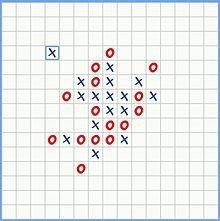
\includegraphics{images/gomoku.jpg}
\end{center}
\\
\textbf{Giới thiệu về cờ Gomoku} \\
Luật chơi của Gomoku như sau:
\begin{itemize}
    \item Bàn cờ 15 x 15, quân đen đi trước.
    \item Lần lượt tới lượt đánh của 2 người đại diện cho quân trắng, quân đen. 
    \item Người chiến thắng là người đầu tiên tạo ra một hàng 5 quân không gián đoạn theo chiều ngang, chiều dọc, hoặc đường chéo.
    \item Các nước Overline, lớn hơn hoặc bằng 6 quân thì không có giá trị với cả 2 bên và không bị coi là lỗi.
\end{itemize}
\begin{center}
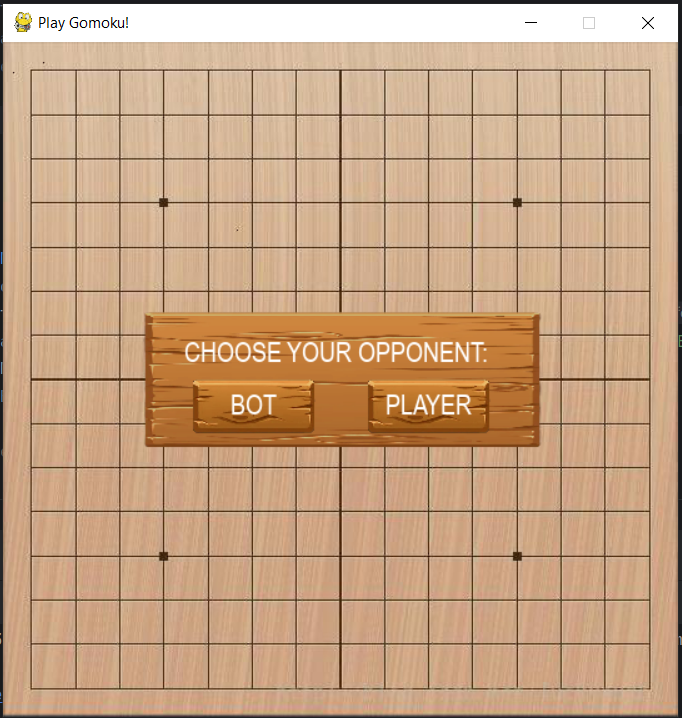
\includegraphics{images/ChoseGameModeGomuku.png} \\
\end{center}
\begin{center}
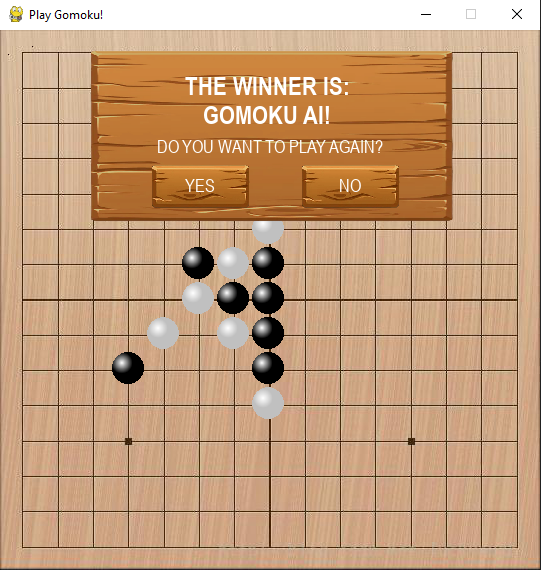
\includegraphics{images/gomoku_AI.png} \\
\end{center}
\textbf{Chức năng đánh với máy}
\begin{itemize}
    \item Sử dụng 2 thuật toán Minimax và Alpha-Beta Pruning để xây dựng bot AI.
    \item Giao diện chơi với máy được thiết kế bằng Pygame.
    \item Người chơi phải chọn màu quân cờ trước khi đánh với máy.
    \item Kết hơp nhiều hàm và các kỹ thuật khác để xây dựng nên một máy có khả năng đánh trả lại khi người chơi đánh một nước cờ. Các hàm chính như: hàm đánh giá, hàm alpha-beta Pruning, hàm kiểm tra chiến thắng, ...
    \item Các nút bấm hay thông báo được định nghĩa bên trong GUI thông qua thư viện Pygame.
\end{itemize}
\begin{center}
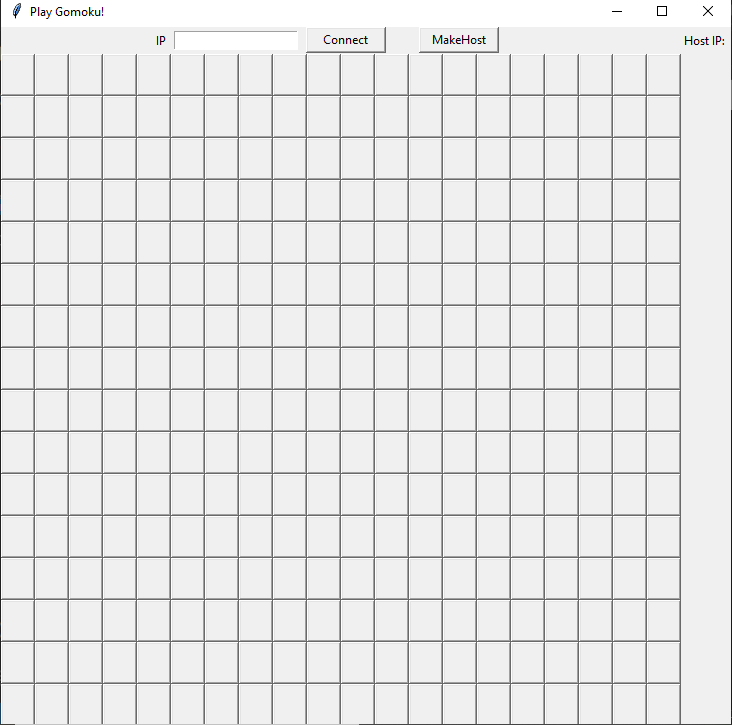
\includegraphics[width=1\textwidth]{images/gomoku_human.png} \\
\end{center}
\textbf{Chức năng đánh với người:}
\begin{itemize}
    \item Giao diện được xây dựng bằng Tkinter
    \item Sử dụng Socket Server cho phép 2 máy tính khác nhau truy cập vào cùng mạng LAN để đánh cờ với nhau.
    \item Nút Make Host: mục đích là tạo ra 1 server thông qua mạng LAN đang truy cập.
    \item Nút Connect: lúc này ở máy tính thứ 2 sẽ đóng vai trò là 1 client cần nhập IP vào input để kết nối tới server đó.
    \item IP của host được hiện trên label góc phải màn hình.
\end{itemize}
\newpage
%%%%%%%%%%%%%%%%%%%%%%%%%%%%%%%%%

\section{DEMO CHƯƠNG TRÌNH}

\subsection{Chức năng chọn chế độ chơi}
    \subsubsection{Giao diện}
    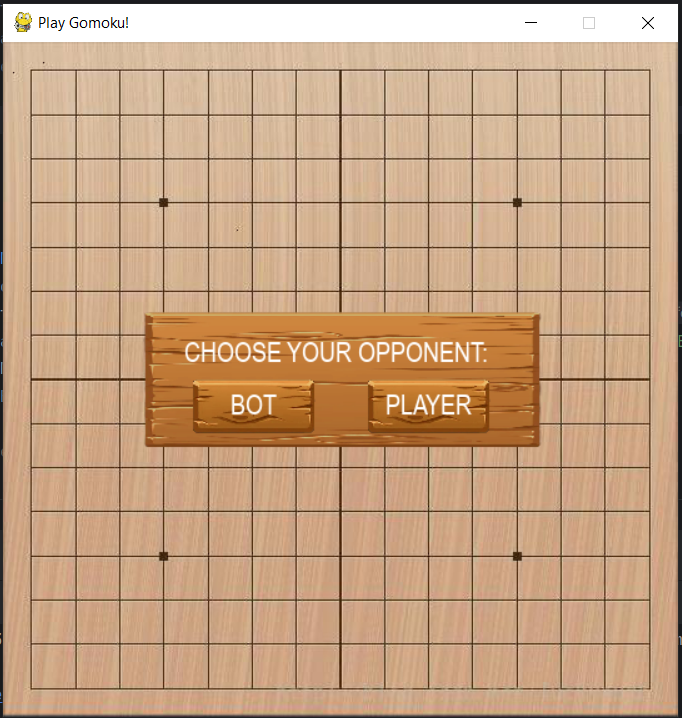
\includegraphics{images/ChoseGameModeGomuku.png}
    \subsubsection{Xử lý}
    \begin{lstlisting}[language=Python]
        from gui.interface import *
        from src.AI import *
        from gui.button import *
        from gui.PvPGUI import *
        import src.utils as utils
        import src.gomoku as gomoku
        import pygame
        
        def ChoseGameMode():
            game = ChooseMode()
            button_bot = Button(game.buttonSurf, 200, 290, "BOT", 22)
            button_player = Button(game.buttonSurf, 340, 290, "PLAYER", 22)
            game.drawMenu()
            game.drawButtons(button_bot, button_player, game.screen)
        
            run = True
            while run:
                for event in pygame.event.get():
                    if event.type == pygame.QUIT:
                        run = False
                    if event.type == pygame.MOUSEBUTTONDOWN \
                            and pygame.mouse.get_pressed()[0]:
                        mouse_pos = pygame.mouse.get_pos()
                        # Check which color the user has chosen and set the states
                        game.checkOpponentChoice(button_bot, button_player, mouse_pos)
                        run = False
            return game

            
        def startGame():
            pygame.init()
            game = ChoseGameMode()
            if game.mode == 1:
                playWithBot()
            elif game.mode == 2:
                Ox = 20  # Số lượng ô theo trục X
                Oy = 20  # Số lượng ô theo trục Y
                window = Window()
                window.showFrame(Ox, Oy)
                window.mainloop()

        
        if __name__ == '__main__':
            startGame()
    \end{lstlisting}
\subsection{Chức năng Đánh với máy}
    \subsubsection{Giao diện}
    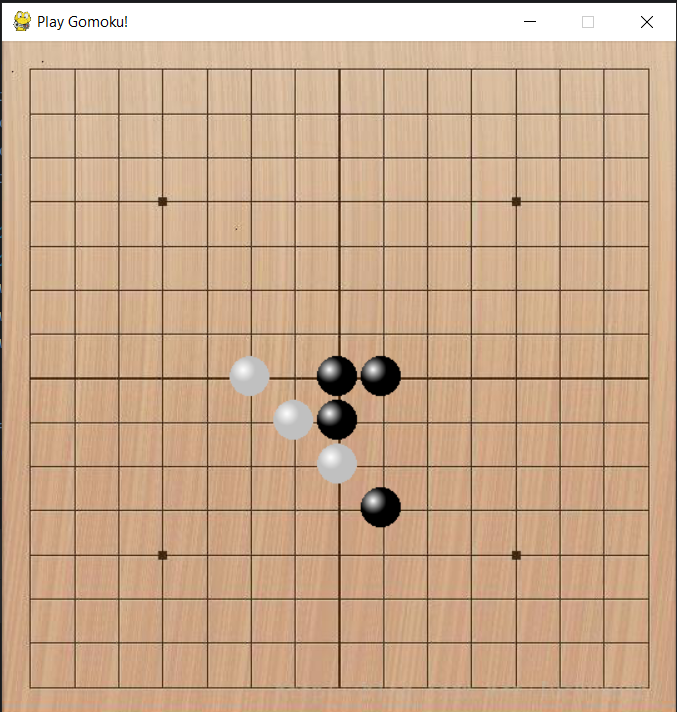
\includegraphics{images/PlayWithBot.png}
    \subsubsection{Xử lý}
    \begin{lstlisting}[language=Python]
        from gui.interface import *
        from src.AI import *
        from gui.button import *
        from gui.PvPGUI import *
        import src.utils as utils
        import src.gomoku as gomoku
        import pygame

        
        def playWithBot():
            # Initializations
            ai = GomokuAI()
            game = GameUI(ai)
            button_black = Button(game.buttonSurf, 200, 290, "BLACK", 22)
            button_white = Button(game.buttonSurf, 340, 290, "WHITE", 22)
        
            # Draw the starting menu
            game.drawMenu()
            game.drawButtons(button_black, button_white, game.screen)
        
            run = True
            while run:
                for event in pygame.event.get():
                    if event.type == pygame.QUIT:
                        run = False
                    if event.type == pygame.MOUSEBUTTONDOWN \
                            and pygame.mouse.get_pressed()[0]:
                        mouse_pos = pygame.mouse.get_pos()
                        # Check which color the user has chosen and set the states
                        game.checkColorChoice(button_black, button_white, mouse_pos)
                        game.screen.blit(game.board, (0, 0))
                        pygame.display.update()
        
                        if game.ai.turn == 1:
                            game.ai.firstMove()
                            game.drawPiece('black', game.ai.currentI, game.ai.currentJ)
                            pygame.display.update()
                            game.ai.turn *= -1
        
                        main(game)
        
                        # When the game ends and there is a winner, draw the result board
                        if game.ai.checkResult() is not None:
                            last_screen = game.screen.copy()
                            game.screen.blit(last_screen, (0, 0))
                            # endMenu(game, last_screen)
                            game.drawResult()
        
                            # Setting for asking the player to restart the game or not
                            yes_button = Button(game.buttonSurf, 200, 155, "YES", 18)
                            no_button = Button(game.buttonSurf, 350, 155, "NO", 18)
                            game.drawButtons(yes_button, no_button, game.screen)
                            mouse_pos = pygame.mouse.get_pos()
                            if yes_button.rect.collidepoint(mouse_pos):
                                # Restart the game
                                game.screen.blit(game.board, (0, 0))
                                pygame.display.update()
                                game.ai.turn = 0
                                startGame()
                            if no_button.rect.collidepoint(mouse_pos):
                                # End the game
                                pygame.quit()
                pygame.display.update()
            endMenu(game, last_screen)
        
        
        def endMenu(game, last_screen):
            pygame.init()
            game.screen.blit(last_screen, (0, 0))
            pygame.display.update()
            run = True
            while run:
                for event in pygame.event.get():
                    game.drawResult()
                    yes_button = Button(game.buttonSurf, 200, 155, "YES", 18)
                    no_button = Button(game.buttonSurf, 350, 155, "NO", 18)
                    game.drawButtons(yes_button, no_button, game.screen)
                    if event.type == pygame.QUIT:
                        run = False
                    if event.type == pygame.MOUSEBUTTONDOWN \
                            and pygame.mouse.get_pressed()[0]:
                        mouse_pos = pygame.mouse.get_pos()
                        if yes_button.rect.collidepoint(mouse_pos):
                            print('Selected YES')
                            game.screen.blit(game.board, (0, 0))
                            pygame.display.update()
                            playWithBot()
                        if no_button.rect.collidepoint(mouse_pos):
                            print('Selected NO')
                            run = False
            pygame.quit()
        
        
        # Main game play loop #
        def main(game):
            pygame.init()
            end = False
            result = game.ai.checkResult()
        
            while not end:
                turn = game.ai.turn
                color = game.colorState[turn]  # black or white depending on player's choice
                for event in pygame.event.get():
                    if event.type == pygame.QUIT:
                        pygame.quit()
        
                    # AI's turn
                    if turn == 1:
                        move_i, move_j = gomoku.ai_move(game.ai)
                        # Make the move and update zobrist hash
                        game.ai.setState(move_i, move_j, turn)
                        game.ai.rollingHash ^= game.ai.zobristTable[move_i][move_j][0]
                        game.ai.emptyCells -= 1
        
                        game.drawPiece(color, move_i, move_j)
                        result = game.ai.checkResult()
                        # Switch turn
                        game.ai.turn *= -1
        
                    # Human's turn
                    if turn == -1:
                        if event.type == pygame.MOUSEBUTTONDOWN \
                                and pygame.mouse.get_pressed()[0]:
                            # Get human move played
                            mouse_pos = pygame.mouse.get_pos()
                            human_move = utils.pos_pixel2map(mouse_pos[0], mouse_pos[1])
                            move_i = human_move[0]
                            move_j = human_move[1]
                            # print(mouse_pos, move_i, move_j)
        
                            # Check the validity of human's move
                            if game.ai.isValid(move_i, move_j):
                                game.ai.boardValue = game.ai.evaluate(move_i, move_j, game.ai.boardValue, -1, game.ai.nextBound)
                                game.ai.updateBound(move_i, move_j, game.ai.nextBound)
                                game.ai.currentI, game.ai.currentJ = move_i, move_j
                                # Make the move and update zobrist hash
                                game.ai.setState(move_i, move_j, turn)
                                game.ai.rollingHash ^= game.ai.zobristTable[move_i][move_j][1]
                                game.ai.emptyCells -= 1
        
                                game.drawPiece(color, move_i, move_j)
                                result = game.ai.checkResult()
                                game.ai.turn *= -1
        
                    if result is not None:
                        # End game
                        end = True
    \end{lstlisting}
\subsection{Chức năng Đánh với người chơi}
    \subsubsection{Giao diện}
    \begin{center}
        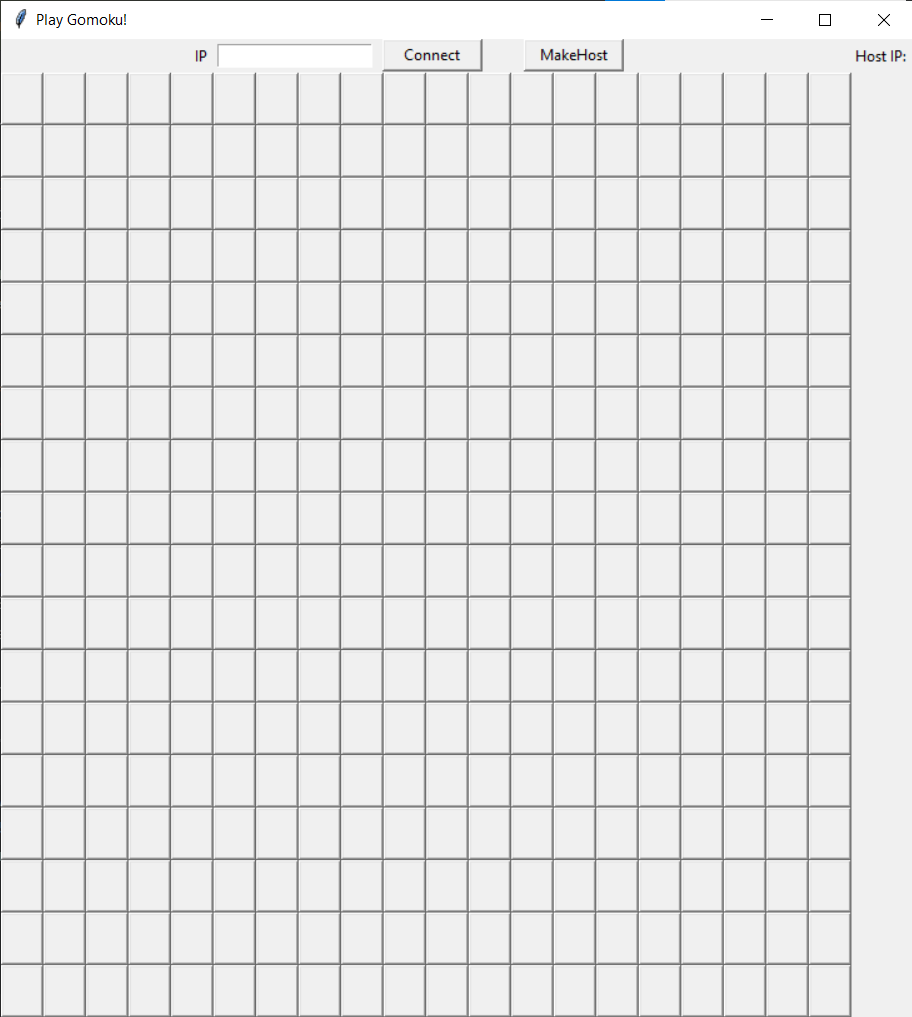
\includegraphics[width=1\textwidth]{images/PlayWithPlayer.png}
    \end{center}
    \subsubsection{Xử lý}
    \begin{lstlisting}[language=Python]
        import tkinter as tk
        from functools import partial
        import threading
        import socket
        from tkinter import messagebox
        
        import pygame
        
        Ox = 20
        Oy = 20
        
        
        class Window(tk.Tk):
            def __init__(self):
                super().__init__()
                self.title("Play Gomoku!")
                self.Buts = {}
                self.current_player = "server"
                self.turn_locked = False
                self.ip_label = tk.Label(self, text="Host IP: ")
                self.ip_label.grid(row=0, column=1, padx=0)
                self.Threading_socket = Threading_socket(self, self.ip_label)
                # Initialize pygame window
                pygame.init()
                self.pygame_screen = pygame.display.set_mode((800, 600))
                print(self.Threading_socket.name)
        
            def showFrame(self, Ox, Oy):
                frame1 = tk.Frame(self)
                frame1.grid(row=0, column=0)
                frame2 = tk.Frame(self)
                frame2.grid(row=1, column=0)
        
                tk.Label(frame1, text="IP", pady=4).grid(row=0, column=1)
                inputIp = tk.Entry(frame1, width=20)  # Khung nhập địa chỉ ip
                inputIp.grid(row=0, column=2, padx=5)
                connectBT = tk.Button(frame1, text="Connect", width=10,
                                      command=lambda: self.Threading_socket.clientAction(inputIp.get()))
                connectBT.grid(row=0, column=3, padx=3)
        
                makeHostBT = tk.Button(frame1, text="MakeHost", width=10,
                                       command=lambda: self.start_server_thread())
                makeHostBT.grid(row=0, column=4, padx=30)
                # Draw pygame board
                for x in range(Ox):
                    for y in range(Oy):
                        self.Buts[x, y] = tk.Button(frame2, font=('arial', 15, 'bold'), height=1, width=2,
                                                    borderwidth=2, command=partial(self.handleButton, x=x, y=y))
                        self.Buts[x, y].grid(row=x, column=y)
        
            def start_server_thread(self):
                thread = threading.Thread(target=self.Threading_socket.serverAction, args=(self.ip_label,))
                thread.start()
        
            def handleButton(self, x, y):
                if self.Buts[x, y]['text'] == '':
                    if not self.turn_locked:
                        if self.current_player == self.Threading_socket.name:
                            self.play_turn(x, y, self.Threading_socket.name)
                            self.turn_locked = True
                            print("Lượt đánh : ", self.current_player)
                        else:
                            print(self.current_player)
                            print(self.Threading_socket.name)
                    else:
                        print("Lượt đánh đã bị khóa.")
                else:
                    pass
        
            def play_turn(self, x, y, player):
                tag = 'O' if player == "server" else 'X'
                self.Buts[x, y]['text'] = tag
                self.Threading_socket.sendData("{}|{}|{}|{}".format("hit", x, y, tag))
                if self.checkWin(x, y, tag, Ox, Oy):
                    self.notification("Winner: ", player)
                    self.newGame(Ox, Oy)
        
            def update_ui(self, x, y, player):
                self.Buts[x, y]['text'] = player
                if player == 'O':
                    self.current_player = "client"
                    winner = 'server'
                elif player == 'X':
                    self.current_player = "server"
                    winner = 'client'
                if self.checkWin(x, y, player, Ox, Oy):
                    self.notification("Winner: ", winner)
                    self.newGame(Ox, Oy)
                self.turn_locked = False
        
            def notification(self, title, msg):
                messagebox.showinfo(str(title), str(msg))
        
            def checkWin(self, x, y, XO, Ox, Oy):
                def checkDirection(dx, dy):
                    count = 1
                    i, j = x + dx, y + dy
        
                    while 0 <= i < Ox and 0 <= j < Oy and self.Buts[i, j]["text"] == XO:
                        count += 1
                        i += dx
                        j += dy
        
                    i, j = x - dx, y - dy
                    while 0 <= i < Ox and 0 <= j < Oy and self.Buts[i, j]["text"] == XO:
                        count += 1
                        i -= dx
                        j -= dy
                    return count >= 5
        
                directions = [(0, 1), (1, 0), (1, 1), (1, -1)]  # Hàng, cột, đường chéo phải, đường chéo trái
        
                for dx, dy in directions:
                    if checkDirection(dx, dy):
                        return True
                return False
        
            def newGame(self, Ox, Oy):
                for x in range(Ox):
                    for y in range(Oy):
                        self.Buts[x, y]['text'] = ''
        
        
        class Threading_socket():
            def __init__(self, gui, ip_label, conn=None):
                super().__init__()
                self.dataReceive = ""
                self.conn = conn
                self.gui = gui
                self.name = ""
                self.ip_label = ip_label
        
            def clientAction(self, inputIP):
                self.name = "client"
                print("client connect ...............")
                HOST = inputIP  
                PORT = 8000  
        
                self.conn = socket.socket(socket.AF_INET, socket.SOCK_STREAM) 
                try:
                    self.conn.connect((HOST, PORT))  
                except ConnectionRefusedError:
                    print("Connection refused. Server may not be available.")
                    return
                self.gui.notification("Đã kết nối tới", str(HOST))
                if inputIP:  # Kiểm tra nếu ip_label được truyền vào
                    self.ip_label.config(text=f"Host IP: {HOST}")  
                t1 = threading.Thread(target=self.client) 
                t1.start()
        
            def serverAction(self, ip_label=None):
                local_ip = get_local_ip()
                self.name = "server"
                HOST = local_ip  # Láy  lập địa chỉ
                print("Make host.........." + HOST)
                if ip_label:  
                    ip_label.config(text=f"Host IP: {HOST}")  
                PORT = 8000 
                s = socket.socket(socket.AF_INET, socket.SOCK_STREAM)
                try:
                    s.bind((HOST, PORT)) 
                    s.listen(2) 
                    self.conn, addr = s.accept() 
                    t2 = threading.Thread(target=self.server, args=(addr, s))
                    t2.start()
                except Exception as e:
                    print("Error:", e)
                    if self.conn:
                        self.conn.close()
                    s.close()
        
            def server(self, addr, s):
                try:
                    print('Connected by', addr)
                    while True:
                        try:
                            self.dataReceive = self.conn.recv(1024).decode()
                            if self.dataReceive != "":
                                action = self.dataReceive.split("|")[0]
                                turn = self.dataReceive.split("|")[3]
                                print(action)
                                if action == "hit" and turn == "X":
                                    x = int(self.dataReceive.split("|")[1])
                                    y = int(self.dataReceive.split("|")[2])
                                    self.gui.update_ui(x, y, turn)
                            self.dataReceive = ""
                        except ConnectionResetError:
                            print("Connection to client reset.")
                            break
                finally:
                    s.close()
            def client(self):
                while True:
                    try:
                        self.dataReceive = self.conn.recv(1024).decode()  
                        if self.dataReceive != "":
                            action = self.dataReceive.split("|")[0]
                            turn = self.dataReceive.split("|")[3]
                            if action == "hit" and turn == "O":
                                x = int(self.dataReceive.split("|")[1])
                                y = int(self.dataReceive.split("|")[2])
                                self.gui.update_ui(x, y, turn)
                                print(action, turn, x, y)
                        self.dataReceive = ""
                    except ConnectionResetError:
                        print("Connection to server reset.")
                        break
        
            def sendData(self, data):
                if self.conn:
                    self.conn.sendall(str(data).encode())
                    print(f"Sent data: {data}")
                else:
                    print("Kết nối không được thiết lập.")
        
        
        def get_local_ip():
            s = socket.socket(socket.AF_INET, socket.SOCK_DGRAM)
            try:
                s.connect(('192.255.255.255', 1))
                IP = s.getsockname()[0]
            except:
                IP = '127.0.0.1'
            finally:
                s.close()
            return IP
        
    \end{lstlisting}
\newpage
%%%%%%%%%%%%%%%%%%%%%%%%%%%%%%%%%

\section{KẾT LUẬN}
\subsection{Tổng kết công việc đã thực hiện}
\begin{itemize}
    \item Nắm bắt cách thức hoạt động của socket dùng trong mạng LAN
    \item Xây dựng được một ứng dụng đánh cờ gomuku với người chơi thông qua mạng LAN
    \item Việc ứng dụng thuật toán Minimax và cải tiến của nó là Alpha-Beta Pruning vào việc xây dựng một bot AI chơi cờ Gomoku là một bước tiến quan trọng trong lĩnh vực trí tuệ nhân tạo và trò chơi. Kết hợp hai phương pháp này giúp bot có thể tính toán các nước đi tiếp theo và đánh giá tình huống hiện tại một cách hiệu quả, từ đó tối ưu hóa quyết định và đảm bảo hiệu suất chơi tốt nhất có thể. 
\end{itemize}
\subsection{Các mặt hạn chế}
\begin{itemize}
    \item Tuy bot AI tạo ra còn chưa hoàn hảo nhưng qua quá trình học tập, nghiên cứu thì em học hỏi được nhiều thứ rất hay về lĩnh vực trí tuệ nhân tạo.
    \item Phương pháp và kiến thức được sử dụng để phát triển đồ án tương đối mới và đa dạng, đặc biệt là Socket server.
\end{itemize}
\subsection{Hướng phát triển tiếp theo trong tương lai}
\begin{itemize}
    \item Tối ưu hóa thuật toán: trong hàm đánh giá ( evaluation function) có thể cải tiến tốt hơn nữa. Bởi vì hàm này dựa vào kinh nghiệm và tư duy của người lập trình. Ngoài ra cần tiếp tục nghiên cứu và tối ưu hóa thuật toán Alpha-Beta Pruning để giảm thời gian tính toán mà vẫn đảm bảo chất lượng nước đi.
    \item Đồng bộ hóa giao diện đánh người với đánh máy nhằm nâng cao trải nghiệm người dùng
\end{itemize}

\end{document}

